\let\negmedspace\undefined
\let\negthickspace\undefined
\documentclass[journal,12pt,twocolumn]{IEEEtran}
\usepackage{cite}
\usepackage{amsmath,amssymb,amsfonts,amsthm}
\usepackage{algorithmic}
\usepackage{graphicx}
\usepackage{textcomp}
\usepackage{xcolor}
\usepackage{txfonts}
\usepackage{listings}
\usepackage{enumitem}
\usepackage{mathtools}
\usepackage{gensymb}
\usepackage[breaklinks=true]{hyperref}
\usepackage{tkz-euclide} % loads  TikZ and tkz-base
\usepackage{listings}
\usepackage{gvv}
%
%\usepackage{setspace}
%\usepackage{gensymb}
%\doublespacing
%\singlespacing

%\usepackage{graphicx}
%\usepackage{amssymb}
%\usepackage{relsize}
%\usepackage[cmex10]{amsmath}
%\usepackage{amsthm}
%\interdisplaylinepenalty=2500
%\savesymbol{iint}
%\usepackage{txfonts}
%\restoresymbol{TXF}{iint}
%\usepackage{wasysym}
%\usepackage{amsthm}
%\usepackage{iithtlc}
%\usepackage{mathrsfs}
%\usepackage{txfonts}
%\usepackage{stfloats}
%\usepackage{bm}
%\usepackage{cite}
%\usepackage{cases}
%\usepackage{subfig}
%\usepackage{xtab}
%\usepackage{longtable}
%\usepackage{multirow}
%\usepackage{algorithm}
%\usepackage{algpseudocode}
%\usepackage{enumitem}
%\usepackage{mathtools}
%\usepackage{tikz}
%\usepackage{circuitikz}
%\usepackage{verbatim}
%\usepackage{tfrupee}
%\usepackage{stmaryrd}
%\usetkzobj{all}
%    \usepackage{color}                                            %%
%    \usepackage{array}                                            %%
%    \usepackage{longtable}                                        %%
%    \usepackage{calc}                                             %%
%    \usepackage{multirow}                                         %%
%    \usepackage{hhline}                                           %%
%    \usepackage{ifthen}                                           %%
  %optionally (for landscape tables embedded in another document): %%
%    \usepackage{lscape}     
%\usepackage{multicol}
%\usepackage{chngcntr}
%\usepackage{enumerate}

%\usepackage{wasysym}
%\documentclass[conference]{IEEEtran}
%\IEEEoverridecommandlockouts
% The preceding line is only needed to identify funding in the first footnote. If that is unneeded, please comment it out.

\newtheorem{theorem}{Theorem}[section]
\newtheorem{problem}{Problem}
\newtheorem{proposition}{Proposition}[section]
\newtheorem{lemma}{Lemma}[section]
\newtheorem{corollary}[theorem]{Corollary}
\newtheorem{example}{Example}[section]
\newtheorem{definition}[problem]{Definition}
%\newtheorem{thm}{Theorem}[section] 
%\newtheorem{defn}[thm]{Definition}
%\newtheorem{algorithm}{Algorithm}[section]
%\newtheorem{cor}{Corollary}
\newcommand{\BEQA}{\begin{eqnarray}}
\newcommand{\EEQA}{\end{eqnarray}}
\newcommand{\define}{\stackrel{\triangle}{=}}
\theoremstyle{remark}
\newtheorem{rem}{Remark}

%\bibliographystyle{ieeetr}
\begin{document}
%

\bibliographystyle{IEEEtran}


\vspace{3cm}

\title{
Question 1.5.7
}
\author{ EE22BTECH11051 - Sreekar Cheela 
}	

% make the title area
\maketitle

\newpage

%\tableofcontents

% Within an equation environment
\begin{flushleft}
	\large Q) Draw a circle with its centre as I (incentre) and radius r (inradius)
	\bigskip
	\large The vertices of the given triangle are:
\end{flushleft}
\\
\begin{align}
	vec {A}= &\myvec{1\\-1};\\ vec {B}= &\myvec{-4\\6};\\ vec {C}= &\myvec{-3\\-5}	
\end{align}
\\
Suppose the equations AB, BC and CA are respectively given by

 \large \begin{align}
    n_{i}^{T} x = c_i , i = 1,2,3
    \end{align}
\\
Then the equations of the angle bisectors are given as 
\\
\begin{align}
     \frac{\lvert n_{i}^{T} x - c_i  \rvert}{\lvert \lvert n_{i} \rvert \rvert} = \pm 
	 \frac{\lvert n_{j}^{T} x - c_j  \rvert}{\lvert \lvert n_{j} \rvert \rvert}
	 i \neq j
\end{align}
 \\
\bigskip 
 From equation (3), we get the angle bisector from B as:
\begin{align}
	&\myvec{
        11 + 7\sqrt{\frac{61}{37}} \\
        1 + 5\sqrt{\frac{61}{37}}			
			}^{T}
			\vec {x} = 2\sqrt{\frac{61}{37}}-38
\end{align}   
\\
 From this equation (3), we get the angle bisector from C as:
\\
\begin{align}
	&\myvec{
		11 + 7\sqrt{61} \\
    	1 - \sqrt{61}
		   }^{T}
		   \vec {x} = 2\sqrt{61}-38
\end{align}

\begin{flushleft}
    The intersection of all the angle bisectors is given as the incentre.
Hence, the incentre can be found by finding the point of intersection of (4) and (5)
\\
The pair of equations can be solved using the augmented matrix $[P \mid Q]$\\
Where P and Q are given as:
\end{flushleft}

\begin{align}
	\text{P=}&\myvec{
		11 + 7\sqrt{\frac{61}{37}} & 1 + 5\sqrt{\frac{61}{37}}\\
		11 + 7\sqrt{61} & 1 - \sqrt{61}
	}
\end{align}

\begin{align}
	\text{Q=}&\myvec{
		2\sqrt{\frac{61}{37}}-38\\
		2\sqrt{61}-38
	}
\end{align}

\begin{align}
	[P \mid Q]=
	\left(
\begin{array}{rr|r}
	11 + 7\sqrt{\frac{61}{37}} & 1 + 5\sqrt{\frac{61}{37}} & 2\sqrt{\frac{61}{37}}-38\\
		11 + 7\sqrt{61} & 1 - \sqrt{61} & 2\sqrt{61}-38
\end{array}
	\right)
\end{align}

\begin{flushleft}
	This augmeneted matrix can be converted into decimal notations for easier calaculations
	and then can be solved using row reductions as follows:
\end{flushleft}
\begin{align*}
	\left(
\begin{array}{rr|r}
	1.81 & 0.67 & -3.21\\
	1.7& -0.62 & -2.03
\end{array}
	\right)
\xleftrightarrow[]{R_2 \leftarrow R_{1} - \frac{1.81}{1.7} R_{2}}
\end{align*}

\begin{align*}
\left(
	\begin{array}{rr|r}
		1.81 & 0.67 & -3.21\\
		0& 1.33 & -1.05
	\end{array}
		\right)
\xleftrightarrow[]{R_{1} \leftarrow R_{1} - \frac{0.67}{1.33} R_{2}}
\end{align*}

\begin{align*}
	\left(
		\begin{array}{rr|r}
			1.81 & 0 & -2.68\\
			0& 1.33 & -1.05
		\end{array}
	\right)
	\xleftrightarrow[]{R_{1} \leftarrow \frac{1}{1.81} R_{1} }
\end{align*}

\begin{align*}
	\left(
		\begin{array}{rr|r}
			1 & 0 & -1.48\\
			0& 1.33 & -1.05
		\end{array}
	\right)
	\xleftrightarrow[]{R_{1} \leftarrow \frac{1}{1.33} R_{1} }
\end{align*}

\begin{align*}
	\left(
		\begin{array}{rr|r}
			1 & 0 & -1.48\\
			0& 1 & -0.79
		\end{array}
	\right)
\end{align*}

\begin{flushleft}
	Hence we get the incentre as:
\end{flushleft}

\begin{align}
	\text{vec{I}=}&\myvec{
		-1.48 \\
		-0.79
	}
\end{align}

\begin{flushleft}
    Now, to find the radius of the incentre, we need to find the distance between 
    the incentre (8) and any one of the sides. 
    \\
    Let us find the distance between BC line and I:
    \\
    BC line equation is given as:
    \bigskip
    \begin{align}
    &\myvec{
        7 \\
        5
	}^{T}	
    \vec {x} = 2
    \end{align}
    \\
    Using the distance formula, we get the radius as:
    \\
    \begin{align}
    r = \frac{185+41\sqrt{37}-37\sqrt{61}-\sqrt{2257}}{6\sqrt{74}}
    \end{align}
    \\Hence the diagram is given as (This diagram has been generated using python):
    \\
\end{flushleft}

\begin{figure}[h]
	\centering
	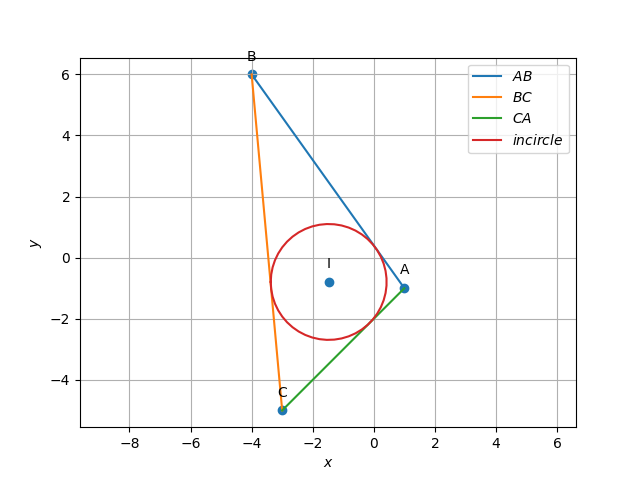
\includegraphics[width=\columnwidth]{./Diagram.png}
	\caption{Triangle with the incircle generated using python}
	\label{Incircle}
\end{figure}

\renewcommand{\thefigure}{\theenumi}
\renewcommand{\thetable}{\theenumi}
%\renewcommand{\theequation}{\theenumi}

\end{document}
